\documentclass[11pt]{article}
\usepackage[utf8]{inputenc}
\usepackage{caption}
\usepackage{amsmath,amsthm,amsfonts,amssymb,amscd}
\usepackage{multirow,booktabs}
\usepackage[table]{xcolor}
\usepackage{fullpage}
\usepackage{lastpage}
\usepackage{enumitem}
\usepackage{pgfplots}
\pgfplotsset{compat=1.18}
\usepackage{fancyhdr}
\usepackage{mathrsfs}
\usepackage{wrapfig}
\usepackage{setspace}
\usepackage{calc}
\usepackage{multicol}
\usepackage{cancel}
\usepackage{tikz}
\usetikzlibrary{positioning}
\usepackage[retainorgcmds]{IEEEtrantools}
\usepackage[margin=3cm]{geometry}
\newlength{\tabcont}
\setlength{\parindent}{0.0in}
\setlength{\parskip}{0.05in}
\usepackage{empheq}
\usepackage{framed}
\usepackage[most]{tcolorbox}

\colorlet{shadecolor}{orange!15}
\geometry{margin=1in, headsep=0.25in}
\theoremstyle{definition}

\newtheorem{defn}{Definition}
\newtheorem{reg}{Rule}
\newtheorem{exer}{Exercise}
\newtheorem{note}{Note}  
\newtheorem*{unnote}{Note} 

\begin{document}
\thispagestyle{empty}

\begin{center}
{\LARGE \bf Lecture Notes}\\
{\large Computer Vision and Pattern Recognition 8820}\\
Spring 2026
\end{center}

\section{Background}
\subsection{Pinhole Camera and Perspective Foreshortening}
Pinhole camera $\rightarrow$ approximation (formed at the focal plane of the camera); this doesn't hold true always.

Perspective Projection $\rightarrow$ used by humans (the model for approximation).

\begin{shaded}
\begin{equation}
\sqrt{
\left(\frac{f x_1}{z} - \frac{f x_2}{z}\right)^2
+
\left(\frac{f y_1}{z} - \frac{f y_2}{z}\right)^2
}
=
\frac{f}{z}
\sqrt{(x_1 - x_2)^2 + (y_1 - y_2)^2}
\end{equation}
\end{shaded}

\noindent
Where $f$ is the camera focal length, $z$ is the depth of the points from the camera, and $(x_1,y_1)$, $(x_2,y_2)$ are their coordinates in the camera frame.

\subsection{Digital Image and Discretization}
In a 2D sensor (CCD Camera), the image intensity is sampled at discrete points in the image plane. The image plane is discretized into cells and pixels (picture elements).

An image is essentially a 2D array (matrix) of cells and pixels. The pixel coordinates $(i, j)$ refer to the center of the cell. The pixel size, essentially the image resolution, can be measured in terms of pixels per unit area.

Discretization of the image plane is equivalent to spatial sampling.

\textbf{Sampling Density/Resolution:} Pixels/Unit area. Higher sampling density leads to higher image resolution. For an image plane of a given area $\rightarrow$ smaller pixel size implies higher resolution.

Digital Image $\rightarrow$ Discretization of spatial coordinates (sampling).

\newpage
\textbf{Discretization of intensity values (Quantization)}

Quantization is the discretization of intensity values. If each pixel is represented using $n$ bits, then the intensity values range from $0$ to $2^{n} - 1$.

\begin{shaded}
For $n = 8$,
\[
\therefore \text{gray-level intensity values} \in \{0, 1, \dots, 255\}.
\]
\end{shaded}

\subsection{Levels of Computation}

\begin{enumerate}
\item \textbf{Pixel Level Computation (contrast enhancement)}
  \begin{itemize}
    \item Output pixel (assume grayscale): Location of pixel or intensity of the pixel.
    \item Each pixel is processed independently (parallelism can be applied; massively data parallel operations).
  \end{itemize}

\item \textbf{Local Level Computation (Parallelizable but not easy) (edge)}
  \begin{itemize}
    \item Output Pixel Value = $f(\text{input pixel value, values of pixels in the neighborhood of the input pixel})$ (overlapping neighborhood).
  \end{itemize}

\item \textbf{Global Level Computation (distance of gray levels within image)}
  \begin{itemize}
    \item Performed on all pixels in image (e.g., Histogram computation).
  \end{itemize}

\item \textbf{Object Level Computation}
  \begin{itemize}
    \item This is performed after a semantic entity is extracted from the image (image region).
    \begin{itemize}
      \item Region Size, Shape, Intensity / Texture.
    \end{itemize}
  \end{itemize}
\end{enumerate}

\newpage
\section{Binary Images}
\subsection{Background}
1 pixel $\rightarrow$ Object Pixel \\
0 pixel $\rightarrow$ non-object pixel (background pixel)

Shape or Geometry Conveyed (e.g., Silhouette of the person). Operations on bits are very efficient (used in robotic sorting).

\textbf{Binary Image Formation:} Created by thresholding a grayscale image.

\subsection{Binary Image Formation (Image Taken)}

\[
B(i,j) = \text{threshold}\big(F(i,j)\big)
\]

\[
\text{threshold}\big(F(i,j)\big) =
\begin{cases} 
1, & \text{if } F(i,j) > T \\
0, & \text{otherwise}
\end{cases}
\]

\textbf{White objects} against dark background.
\begin{unnote}
Selection of \textbf{T} is based on \textbf{domain knowledge}.
\end{unnote}

\newpage
\section{Geometric Properties of Interest}
\subsection{Object Size}
\begin{unnote}
Assumption: image contains one object.
\end{unnote}
\begin{enumerate}
    \item \textbf{Object Size:}
    \begin{equation}
    A = \sum_{i=1}^{n} \sum_{j=1}^{m} B(i, j)
    \end{equation}
    \item \textbf{Centroid:}
    \begin{equation}
    X_C = \frac{1}{A}\sum_{i=1}^n\sum_{j=1}^m j \cdot B(i,j), \quad Y_C = \frac{1}{A}\sum_{i=1}^n\sum_{j=1}^m i \cdot B(i,j)
    \end{equation}
    \item \textbf{Orientation of Object:}
    Normalizing the coordinates based on the centroid:
    \[x' = j - x_c, \quad y' = i - y_c\]
    Centralized coordinates w.r.t. centroid:
    \begin{equation}
    a = \sum_{i=1}^{n} \sum_{j=1}^{m} [x' (i, j)]^2 B(i, j) 
    \end{equation}
\end{enumerate}

\section{Moments}
\subsection{Object Orientation}
To compute the second-order moments $a$, $b$, and $c$, we start with the equation:
\[
\tan(2\theta) = \frac{b}{a-c}
\]

\newpage
\begin{shaded}
    \begin{equation}
        a = \sum_{i=1}^{n}\sum_{j=1}^{m}[X^\prime(i,j)]^2 \cdot B(i,j)
    \end{equation}
    \begin{equation}
        b = 2\sum_{i=1}^{n}\sum_{j=1}^{m}[X^\prime(i,j)][Y^\prime(i,j)] \cdot B(i,j)
    \end{equation}
    \begin{equation}
        c = \sum_{i=1}^{n}\sum_{j=1}^{m}[Y^\prime(i,j)]^2 \cdot B(i,j)
    \end{equation}
\end{shaded}

Consider the following expression for $X^2$ (moment of inertia):
\begin{equation}X^2 = \frac{1}{2}(a+c) + \frac{1}{2}(a-c) \cos(2\theta) + \frac{b}{2} \sin(2\theta)\end{equation}

\textbf{Substitution Step:}
We substitute $2\theta_1$ and $2\theta_2$ into the expression for $X^2$. The value of $X^2$ is minimized for one and maximized for the other. The axis of orientation is the one that minimizes $X^2$.

\textbf{Elongation:}
The elongation ratio is given by $E = \frac{X_{\text{max}}}{X_{\text{min}}}$. For a \textbf{sphere}, the elongation is $E = 1$.

\subsection{Projections}
\begin{equation}
    H[i] = \sum_{j=1}^{m} B(i, j), \quad V[j] = \sum_{i=1}^{n} B(i, j)
\end{equation}
Where $H$ and $V$ are compact representations of $B(i,j)$.

\newpage
\section{Topological Definitions}
\subsection{Path}
A sequence of pixels where successive pixels are neighbors.
\begin{itemize}
    \item 4-path $\rightarrow$ successive pixels are 4-neighbors.
    \item 8-path $\rightarrow$ successive pixels are 8-neighbors.
\end{itemize}

\subsection{Foreground}
The set of pixels with value 1, denoted by $S$.

\subsection{Connectivity}
A pixel $p \in S$ is connected to pixel $q \in S$ if there exists a path from $p$ to $q$ consisting entirely of pixels in $S$.

\subsection{Relations}
\begin{itemize}
    \item $p$ is trivially connected to $p$ (reflexive).
    \item $p$ is connected to $q \iff q$ is connected to $p$ (symmetric).
    \item If $p$ is connected to $q$ and $q$ is connected to $r$, then $p$ is connected to $r$ (transitive).
\end{itemize}

The connectivity relation partitions $S$ into connected components ($S_1, S_2, \dots$):
\begin{itemize}
\item $\bigcup S_i = S$
\item $S_i \cap S_j = \emptyset \quad \forall i \neq j$
\end{itemize}

\newpage
\section{Image Segmentation}
Let $\bar{S}$ = complement of $S$ (set of 0-pixels). The set of all connected components of $\bar{S}$ that have pixels on the image border are referred to as the \textbf{background}. Other components of $\bar{S}$ are referred to as \textbf{holes}.

\subsection{Criteria/Caveat}
Different criteria need to be used for $S$ and $\bar{S}$ in terms of connectivity to avoid paradoxes.

$S'_{int} = S' - S'_{boundary}$

\textbf{Surrounded / Contains Relation:}
A set of pixels $T$ is said to surround a set of pixels $S$ if any 4-path from any pixel of $S$ to the image border must intersect $T$. If $T$ surrounds $S$, then $S$ is contained in $T$.

\newpage
\section{Connected Component Labeling (CCL)}
The process of assigning a unique label to each connected component in $S$.

\subsection{Recursive CCL Algorithm}
\begin{itemize}
\item Scan the image until an unlabeled 1-pixel is found and assign it a new label $L$.
\item Assign recursively the label $L$ to all of its neighboring 1-pixels.
\item Halt recursion when no more unlabeled 1-pixels are found.
\item Repeat until no more unlabeled 1-pixels exist.
\end{itemize}

\subsection{Iterative (Sequential) CCL Algorithm}
1. \textbf{Raster Scan:} Left to right, top to bottom. \\
2. \textbf{Serpentine Scan:} Lawn mower scan.

\textbf{4CC Iterative Process:}
1. Raster scan the image.
2. If the given pixel $p$ is a 1-pixel:
    \begin{itemize}
        \item If only one of $u$ (upper) or $l$ (left) has a label, assign it to $p$.
        \item If both have the same label, assign it to $p$.
        \item If they have different labels, assign $p$ the label of $u$ and record equivalence.
        \item If neither has a label, create a new label.
    \end{itemize}
3. Second pass: Re-assign pixels to a unique label from their equivalence class.

\newpage
\section{Boundary Extraction}
Binary Image $\rightarrow$ CCL $\rightarrow$ Size Filtering.

\textbf{Size Filtering:} Replace all components where Area $< T$ with 0.

\textbf{Euler Number:} $E = n.components - n.holes$.

\textbf{Boundary Extraction Algorithm:}
1. Raster scan to find starting pixel.
2. Current pixel $\leftarrow$ starting pixel; $b \leftarrow$ 4-neighbor to the west.
3. Enumerate 8-neighbors $n_1 \dots n_8$ clockwise starting from $b$.
4. Determine smallest $i$ such that $n_i$ belongs to component.
5. Append pixel to contour list. Update $b$ and current pixel.
6. Repeat until returning to starting pixel.

\textbf{Boundary Properties:}
1. \textbf{Perimeter (8-connected):} 4-neighbors add 1, diagonal neighbors add $\sqrt{2}$.
2. \textbf{Compactness:} $Compactness = \frac{Perimeter^2}{Area}$. Circles have the smallest compactness ($4\pi$).

\section{Skeletonization of a 2D Shape}
\subsection{Distance Measure Properties}
A distance function $d(p,q)$ satisfies:
\begin{itemize}
\item Non-negativity: $d(p,q) \ge 0$
\item Identity: $d(p,q) = 0 \iff p = q$
\item Symmetry: $d(p,q) = d(q,p)$
\item Triangle inequality: $d(p,r) \le d(p,q) + d(q,r)$
\end{itemize}

\subsection{Distance Measures}
1. \textbf{Euclidean:} $d_E(p,q) = \sqrt{(i_1 - i_2)^2 + (j_1 - j_2)^2}$
2. \textbf{Chessboard:} $d_C(p,q) = \max(|i_1 - i_2|, |j_1 - j_2|)$

\newpage
\section{Skeletonization (Cont.)}
The distance transform (DT) of $S$ is the minimum distance from each pixel in $S$ to the background $\bar{S}$.

\subsection{Medial Axis Transform (MAT)}
\begin{shaded}
    \begin{equation}
        \text{MAT}(i, j) = \begin{cases}   1, & \text{if } DT(i, j) \geq DT(u, v) \text{ for all } (u, v) \in N(i, j) \\   0, & \text{otherwise} \end{cases}
    \end{equation}
\end{shaded}
The original component can be reconstructed from MAT using reverse distance propagation.

\section{Region Analysis in Grayscale Images}
\subsection{Formal Definition of Image Segmentation}
Partition image $I$ into $R_1 \dots R_n$ such that:
\begin{shaded}
    \begin{equation}
        \bigcup_{i=1}^{n} R_i = I \quad (\text{exhaustive})
    \end{equation}
    \begin{equation}
        R_i \cap R_j = \emptyset \quad \forall i \neq j \quad (\text{exclusive})
    \end{equation}
\end{shaded}

\subsection{Approaches}
1. \textbf{Region Based (Similarity):} Group pixels that belong to a single object.
2. \textbf{Edge Based (Dissimilarity):} Detect edge pixels and construct boundaries.

\newpage
\section{Modal Analysis}
\subsection{Iterative Threshold Selection}
1. Initial estimate $T$ = average intensity of the image.
2. Partition into $R_1, R_2$ using $T$.
3. Compute means $\mu_1, \mu_2$.
4. $T_{new} = \frac{\mu_1 + \mu_2}{2}$. Repeat until convergence.

\subsection{Non-Uniform Background (Variable Thresholding)}
Used when background variation is systematic.
\[ F_n(x,y) = F(x,y) - F'(x,y) \]
$F'$ is obtained via regression (Bilinear, Biquadratic, Bicubic).

\section{Adaptive Thresholding}
1. Divide image into sub-images.
2. Threshold independently.
3. Combine results (can lead to artifacts/mosaic effect).

\begin{center}
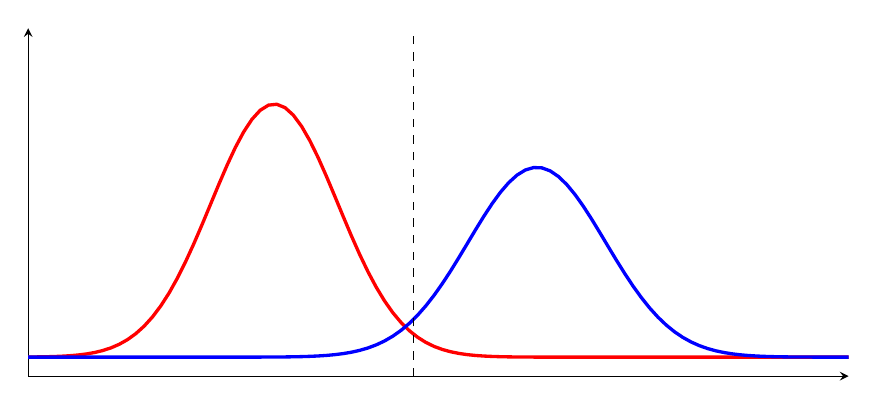
\begin{tikzpicture}
\begin{axis}[
    width=12cm, height=6cm, xmin=0, xmax=10, ymin=0,
    axis lines=left, xtick=\empty, ytick=\empty,
    samples=100, domain=0:10,
]
\addplot[red, very thick] {0.12 + 1.6*exp(-((x-3.0)^2)/1.2)};
\addplot[blue, very thick] {0.12 + 1.2*exp(-((x-6.2)^2)/1.4)};
\addplot[black, dashed] coordinates {(4.7,0) (4.7,2.2)};
\end{axis}
\end{tikzpicture}
\end{center}

\section{Dual Thresholding with Region Growing}
1. Select $T_1, T_2$.
2. Classify: $R_1$ (Foreground), $R_2$ (Background), $R_3$ (Uncertain).
3. If $R_3$ pixel has a neighbor in $R_1$, reassign to $R_1$.
4. Repeat until stable. Use spatial coherence to reduce misclassification.

\newpage
\section{Region Representation Schemes}
1. \textbf{Label Array:} $L(i,j) = \alpha$.
2. \textbf{Bitmap (Mask):} $\beta^{\alpha}(i,j) = 1$ if pixel belongs to $\alpha$.
3. \textbf{Hierarchical:} Image Pyramid (FOA - Focus of Attention).

\section{QuadTree / OctTree}
Leaf nodes represent homogeneous regions. If not homogeneous, split into 4 (Quad) or 8 (Oct) children.

\section{Region Adjacency Graph (RAG)}
\begin{itemize}
    \item \textbf{Nodes:} Represent Regions (Attributes: geometry, spectral).
    \item \textbf{Arcs:} Represent common boundaries (Attributes: contour properties).
\end{itemize}

\section{Split and Merge Segmentation}
1. \textbf{Split Phase:} If node fails homogeneity test (e.g., high variance), split.
2. \textbf{Merge Phase:} If adjacent nodes are similar, merge.
Iterate until no changes occur.

\section{Iterative Model Fitting}
Fit a parametric function $f(x, y, a, m) = \sum a_{ij} x^i y^j$.
\begin{equation}
X^2(R, a, m) = \sum_{(x,y)\in R} \left[ F(x, y) - f(x, y, a, m) \right]^2
\end{equation}
Seed regions are grown based on fitting error thresholds.

\section{Edge Detection}
Edge: Location of significant change in local property (gray level, color, texture, motion).

\textbf{Signal-to-Noise Ratio (SNR):} $SNR = \frac{A_s^2}{A_n^2}$.
Edge detection is preceded by smoothing to reduce noise variance ($Var = \sigma^2/k$).

\section{Averaging Filter}
\[
I_{s} (i, j) = \sum_{k=-\frac{M-1}{2}}^{\frac{M-1}{2}} \sum_{l=-\frac{M-1}{2}}^{\frac{M-1}{2}} W(k,l) I(i+k, j+l)
\]

For a smoothing filter:
\begin{itemize}
    \item [A.] $W(k,l) \ge 0$
    \item [B.] $\sum \sum W(k, l) = 1$
\end{itemize}

Given image $I_1$ and filter $W$ of size $M \times M$ where $M$ is odd:
\begin{equation}
I_{1S}(i,j) = \sum_{k=-\frac{M-1}{2}}^{\frac{M-1}{2}} \sum_{l=-\frac{M-1}{2}}^{\frac{M-1}{2}} W(k,l)\, I_1(i+k, j+l)
\end{equation}

\[
I_{1S} = W \circledast I_1
\]

\textbf{Key Insight:}  
A smoothing filter is a linear operator.

\section{Noise}
Gaussian Noise can be smoothed out by a convolution filter. Blurring is essentially uncertainty localization.



\subsection{Salt and Pepper Noise (Impulse Noise)}
Noise takes two extreme values:
\begin{itemize}
    \item[-] Min 0 (pepper)
    \item[-] Max 255 (salt)
\end{itemize}

\begin{align}
I(i,j) &= \text{Min} && \text{with probability } p \\
I(i,j) &= \text{Max} && \text{with probability } g \\
I(i,j) &= I(i,j) && \text{with probability (unchanged) } 1-p-g
\end{align}



\end{document}